\section{Gehäuse für Platine}
Momentan wird die Platine mit Hilfe von Heißkleber ohne Gehäuse in der Station fixiert.
\ac{eagle} bietet in der neuesten Version eine Exportfunktion in die A360-Cloud von Autodesk an, mit welcher die Platine inklusive der verwendeten Bauteile als 3D-Modell exportiert werden kann.
Dieses Modell kann in dafür geeigneten Autodesk-Programmen wie Fusion 360 geöffnet und für die Planung eines Gehäuses verwendet werden.
\begin{figure}[htbp!]
	\centering
	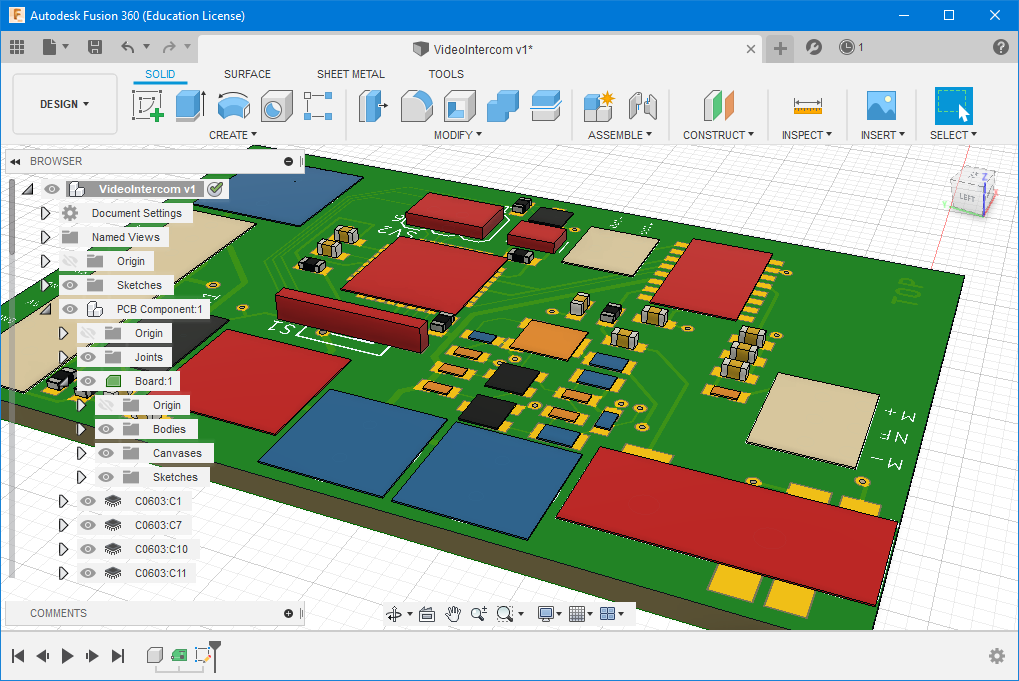
\includegraphics[width=.9\linewidth]{images/hardware-ausblick/fusion360.png}
	\caption{Exportierte Platine in Fusion 360}
\end{figure}

\section{Platine Version 2}
Die im Zuge dieser Diplomarbeit entwickelte Platine ist zwar voll funktionsfähig, jedoch bedarf es weiterer Verbesserungen.
Zum einen wurden aufgrund von Miskommunikation die Anschlüsse, die zum Programmieren notwendig sind, falsch verdrahtet. Die zweite Version des Platinendesigns würde dieses Problem beheben.
Zusätzlich zu den bereits vorhandenen Anschlüssen sollen in der zweiten Version noch ein paar zusätzliche digitale \acp{io} hinzugefügt werden, um die Diebstahlsicherung der Außenstation auswerten zu können. Die Software würde diese Funktionalität bereits teilweise unterstützen.
Die zweite Platinenversion ist bereits vollständig geplant, allerdings noch nicht gefertigt worden.
